\documentclass[
  bibliography=totoc,     % Literatur im Inhaltsverzeichnis
  captions=tableheading,  % Tabellenüberschriften
  titlepage=firstiscover, % Titelseite ist Deckblatt
]{scrartcl}

% Paket float verbessern
\usepackage{scrhack}

% Warnung, falls nochmal kompiliert werden muss
\usepackage[aux]{rerunfilecheck}

% unverzichtbare Mathe-Befehle
\usepackage{amsmath}
% viele Mathe-Symbole
\usepackage{amssymb}
% Erweiterungen für amsmath
\usepackage{mathtools}

% Fonteinstellungen
\usepackage{fontspec}
% Latin Modern Fonts werden automatisch geladen
% Alternativ zum Beispiel:
%\setromanfont{Libertinus Serif}
%\setsansfont{Libertinus Sans}
%\setmonofont{Libertinus Mono}

% Wenn man andere Schriftarten gesetzt hat,
% sollte man das Seiten-Layout neu berechnen lassen
\recalctypearea{}

% deutsche Spracheinstellungen
\usepackage[ngerman]{babel}


\usepackage[
  math-style=ISO,    % ┐
  bold-style=ISO,    % │
  sans-style=italic, % │ ISO-Standard folgen
  nabla=upright,     % │
  partial=upright,   % ┘
  warnings-off={           % ┐
    mathtools-colon,       % │ unnötige Warnungen ausschalten
    mathtools-overbracket, % │
  },                       % ┘
]{unicode-math}

% traditionelle Fonts für Mathematik
\setmathfont{Latin Modern Math}
% Alternativ zum Beispiel:
%\setmathfont{Libertinus Math}

\setmathfont{XITS Math}[range={scr, bfscr}]
\setmathfont{XITS Math}[range={cal, bfcal}, StylisticSet=1]

% Zahlen und Einheiten
\usepackage[
  locale=DE,                   % deutsche Einstellungen
  separate-uncertainty=true,   % immer Unsicherheit mit \pm
  per-mode=symbol-or-fraction, % / in inline math, fraction in display math
]{siunitx}

% chemische Formeln
\usepackage[
  version=4,
  math-greek=default, % ┐ mit unicode-math zusammenarbeiten
  text-greek=default, % ┘
]{mhchem}

% richtige Anführungszeichen
\usepackage[autostyle]{csquotes}

% schöne Brüche im Text
\usepackage{xfrac}

% Standardplatzierung für Floats einstellen
\usepackage{float}
\floatplacement{figure}{htbp}
\floatplacement{table}{htbp}

% Floats innerhalb einer Section halten
\usepackage[
  section, % Floats innerhalb der Section halten
  below,   % unterhalb der Section aber auf der selben Seite ist ok
]{placeins}

% Seite drehen für breite Tabellen: landscape Umgebung
\usepackage{pdflscape}

% Captions schöner machen.
\usepackage[
  labelfont=bf,        % Tabelle x: Abbildung y: ist jetzt fett
  font=small,          % Schrift etwas kleiner als Dokument
  width=0.9\textwidth, % maximale Breite einer Caption schmaler
]{caption}
% subfigure, subtable, subref
\usepackage{subcaption}

% Grafiken können eingebunden werden
\usepackage{graphicx}

% schöne Tabellen
\usepackage{booktabs}

% Verbesserungen am Schriftbild
\usepackage{microtype}

% Literaturverzeichnis
\usepackage[
  backend=biber,
]{biblatex}
% Quellendatenbank
\addbibresource{lit.bib}
\addbibresource{programme.bib}

% Hyperlinks im Dokument
\usepackage[
  german,
  unicode,        % Unicode in PDF-Attributen erlauben
  pdfusetitle,    % Titel, Autoren und Datum als PDF-Attribute
  pdfcreator={},  % ┐ PDF-Attribute säubern
  pdfproducer={}, % ┘
]{hyperref}
% erweiterte Bookmarks im PDF
\usepackage{bookmark}

% roemische Zahlen
 \usepackage{romannum} 

% Trennung von Wörtern mit Strichen
\usepackage[shortcuts]{extdash}

\author{%
  Philip Jaletzky\\%
  \href{mailto:philip.jaletzky@udo.edu}{philip.jaletzky@udo.edu}%
  \and%
  Matthias Maile\\%
  \href{mailto:matthias.maile@udo.edu}{matthias.maile@udo.edu}%
}
\publishers{TU Dortmund – Fakultät Physik}


\subject{V601}
\title{Franck-Hertz-Versuch}
\date{%
  Durchführung: 29.06.2021
  \hspace{3em}
  Abgabe: 06.07.2021
}

\begin{document}
\pagenumbering{arabic} % damit Seitenzahlen nicht roemisch sind

\maketitle
\thispagestyle{empty}
\tableofcontents
\newpage

\section{Theorie}
\label{sec:Theorie}
Im vorliegenden Versuch wurde das Relaxationsverhalten eines RC-Stromkreises untersucht.

\subsection{Anwendung einer allgemeinen Relaxationsgleichung auf den RC-Kreis}

Generell treten Relaxationsphänomene in der Physik auf, wenn ein System aus seinem Ausgangszustand ausgelenkt wird und anschließend (ohne Oszillation) in diesen Ausgangszustand zurückkehrt. Dabei ist die Änderung der betrachteten Größe zu einer bestimmten Zeit in der Regel proportional zu der Differenz der Größe von ihrem Endzustand. Die Änderung der Größe A kann also mit der Gleichung
\begin{equation}
    \frac{\text{d}A}{\text{d}t} = c \left[A(t) - A(\infty) \right]
    \label{eqn:Relaxation}
\end{equation}
berechnet werden. Eine Umformung (Trennung von dA und dt) und Integration von \autoref{eqn:Relaxation} über die Zeit von 0 bis t ergibt
\begin{equation}
    ln(\frac{A(t) - A(\infty)}{A(0) - A(\infty)}) = c t \text{.}
    \label{eqn:RelaxationInt}
\end{equation}
Die Umformung von \autoref{eqn:RelaxationInt} nach $A(t)$ liefert schließlich 
\begin{equation}
    A(t)= A(\infty)+(A(0) - A(\infty)) e^{c t} \text{.}
    \label{eqn:Auslenkung}
\end{equation}

Als Beispiele für solche Relaxationsvorgänge werden nun die Ent- und die Aufladung eines Kondensators über einen Widerstand betrachtet (siehe \autoref{fig:entaufladung}).
\begin{figure}
    \centering
    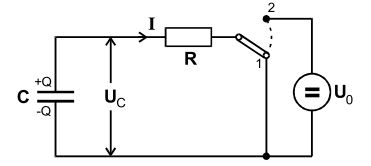
\includegraphics{images/entaufladung.JPG}
    \caption{Beispielschaltung zur Entladung (Stellung 1) und Aufladung (Stellung 2) eines Kondensators über einen Widerstand \cite{VA}}
    \label{fig:entaufladung}
\end{figure}

\textbf{Entladung}:
Wie in \autoref{fig:entaufladung} zu sehen, befindet sich auf den Platten des Kondensators mit Kapazität C die Ladung Q, sodass zwischen den Platten die Spannung $U_C$ liege, die nach 
\begin{equation}
    U_C = \frac{Q}{C}
    \label{eqn:U}
\end{equation}

berechnet werden kann. Das ohmsche Gesetz liefert nun den Strom I durch den Widerstand R, der durch die Spannung hervorgerufen wird:
\begin{equation}
    I =   \frac{U_C}{R}
    \label{eqn:I}
\end{equation}
Der Strom I bewirkt einen Ladungsfluss, sodass sich die Ladung auf den Kondensatorplatten im Zeitintervall dt um
\begin{equation}
    \text{d}Q = -I \text{d}t
    \label{eqn:dQ}
\end{equation}
ändert. Mit \autoref{eqn:U}, \autoref{eqn:I} und \autoref{eqn:dQ} kann nun eine Differentialgleichung für die Ladung auf den Kondensatorplatten $Q(t)$ aufgestellt werden, die die gleiche Form wie \autoref{eqn:Relaxation} hat:
\begin{equation}
        \frac{\text{d}Q}{\text{d}t}  = - \frac{1}{RC} Q(t) 
\end{equation}

Für die Entladung kann angenommen werden, dass $Q(\infty)=0$ gilt. Dann liefert \autoref{eqn:Auslenkung} hier \newline
\begin{equation}
    Q(t)= Q(0) e^{\frac{-t}{RC}} \text{.}
    \label{eqn:Qentl}
\end{equation}


\textbf{Aufladung}:
Der Aufladevorgang des Kondensators kann analog betrachtet werden. Für die Aufladung gelten die Randbedingungen $Q(0)=0$ und $Q(\infty)=CU_0$. Für den zeitlichen Verlauf der Ladung ergibt sich hier also (siehe auch \autoref{eqn:Auslenkung}):
\begin{equation}
    Q(t)= CU_0 (1-e^{\frac{-t}{RC}}) 
    \label{eqn:Qaufl}
\end{equation}
Der Ausdruck $RC$ wird auch als Zeitkonstante des Relaxationsvorganges bezeichnet.

\subsection{Relaxation unter periodischer Auslenkung aus der Gleichgewichtslage}
Die unter periodischer Auslenkung auftretenden Relaxationsphänomene eines RC-Stromkreises werden nun beispielhaft anhand der Schaltung in \autoref{fig:schaltung} betrachtet.

\begin{figure}
    \centering
    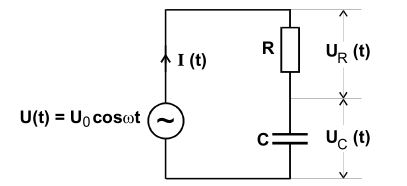
\includegraphics{images/Schaltung.JPG}
    \caption{Beispielschaltung für einen RC-Kreis mit periodischer Anregung \cite{VA}}
    \label{fig:schaltung}
\end{figure}
Wenn die Kreisfrequenz $ \omega << 1/RC$ ist, ist die äußere Wechselspannung  
\begin{equation}
    U(t) = U_0 \cdot \text{cos}(\omega t)
\end{equation}
zu jedem Zeitpunkt praktisch gleich der Spannung am Kondensator $U_C$. Bei steigender Frequenz entsteht allerdings eine Phasenverschiebung zwischen Generator- und Kondensatorspannung, außerdem sinkt die Amplitude der Kondensatorspannung. Im Folgenden werden Formeln für die Frequenzabhängigkeit der Phase $\varphi(\omega)$ und der Amplitude $A(\omega)$ hergeleitet. Für die genauere Betrachtung dieses Zusammenhangs wird der Ansatz
\begin{equation} 
    U_\text{C}(t) = A(\omega) \text{cos}(\omega t + \varphi(\omega))
    \label{eqn:ansatz}
\end{equation}
gewählt.
Mit dem 2. Kirchhoffschen Gesetz (Maschenregel) gilt für die Schaltung in \autoref{fig:schaltung}
\begin{align}
    \label{eqn:Uta}
    U(t) &= U_R(t) + U_C(t) \\
    \iff     U_0 \cos(\omega t) &= I(t)R +A(\omega) \cos(\omega t + \varphi) 
    \label{eqn:Ut}
\end{align}
und mit \autoref{eqn:U} und \autoref{eqn:dQ} kann man die Stromstärke als
\begin{equation}
    \label{eqn:Stromstaerke}
    I(t) = \frac{\text{d}Q}{\text{d}t} = C \cdot \frac{\text{d}U_\text{C}}{\text{d}t}
\end{equation}
schreiben. Das Einsetzen von \autoref{eqn:ansatz} und \autoref{eqn:Stromstaerke} in \autoref{eqn:Ut} ergibt dann die Gleichung

\begin{equation}
    \label{eqn:gl}
        U_0 \cos(\omega t) = -A  \omega RC \sin(\omega t + \varphi)+
        A \cos(\omega t + \varphi)   \text{.}  
\end{equation}

Aus \autoref{eqn:gl} wird für $\omega t = \frac{\pi}{2}$  
\begin{equation}
    0= - \omega RC \sin(\frac{\pi}{2}+\varphi)+\cos(\frac{\pi}{2}+\varphi)
    \label{eqn:pihalbe}
\end{equation}
und dies kann umgeformt werden zu (mit $\sin(\varphi + \frac{\pi}{2}) = \cos \varphi$ und $\cos(\varphi + \frac{\pi}{2}) = - \sin (\varphi)$):

\begin{align}
    \label{eqn:Phase1}
    \frac{\sin(\varphi)}{\cos(\varphi)} = \tan(\varphi) &= - \omega RC \\
    \iff \varphi(\omega) &= \arctan(- \omega RC)
    \label{eqn:Phase}
\end{align}

Mit $\omega t + \varphi =\frac{\pi}{2}$ kann \autoref{eqn:gl} auch zu 
\begin{align}
        U_0 \cos(\frac{\pi}{2} - \varphi) &= -A  \omega RC \\
        \iff A(\omega) &= - \frac{\sin(\varphi)}{\omega RC} U_0
        \label{eqn:gl1}
    \end{align}
umgeformt werden. Aus \autoref{eqn:Phase1} wird dann unter Benutzung des trigonometrischen Pythagoras (man ersetze beispielsweise $\cos(\varphi)$ durch $\sqrt{1-\sin(\varphi)^2}$)
\begin{equation}
    \sin(\varphi) = \frac{\omega R C}{\sqrt{1 + (\omega RC)^2}}.
    \label{eqn:sin}
\end{equation}
hergeleitet. Schließlich erhält man durch Einsetzen von \autoref{eqn:sin} in \autoref{eqn:gl1}
\begin{equation}
    A(\omega) = \frac{U_0}{\sqrt{1 + \omega^2 R^2 C^2}}.
    \label{eqn:Amplitude}
\end{equation}


Mit \autoref{eqn:Phase} und \autoref{eqn:Amplitude} wurden also Formeln für die Frequenzabhängigkeit der Phase und der Amplitude hergeleitet.

\subsection{RC-Kreis als Integrator}
Unter bestimmten Voraussetzungen kann ein RC-Kreis auch als Integrator dienen. Das heißt, dass er eine zeitlich veränderliche Eingangsspannung integriert. Mit \autoref{eqn:Uta} und \autoref{eqn:Stromstaerke} erhält man:
\begin{equation}
    U(t) = RC \frac{\text{d}U_\text{C}}{\text{d}t} + U_\text{C}(t) 
\label{eqn:ut}
\end{equation} 

Die Voraussetzung ist hier, dass $ω >> 1/RC$ ist, dann ist  $|U_C|<<|U_R|$ und $|U_C|<<|U|$. Daher wird \autoref{eqn:ut} näherungsweise zu:

\begin{align}
U(t) &= RC \cdot \frac{\text{d}U_\text{C}}{\text{d}t} \\
\iff U_\text{C}(t) &= \frac{1}{RC} \int^t_0 U(t') \; \text{d} t'
\end{align}
\section{Durchführung}
\label{sec:Durchführung}
Im Folgenden soll auf die Durchführung der Messung eingegangen werden. Die gesamte
Messreihe wird dabei mit zwei verschiedenen Pendellängen durchgeführt. In beiden sollen
folgende Werte bestimmt werden:
\begin{itemize}
	\item Die Schwingungsdauern der einzelnen Pendel frei schwingend $T_i$,
	\item Die Schwingungsdauer $T_+$ der gleichphasigen Schwingung,
	\item $T_-$ für gegenphasige Schwingung,
	\item Schwingungsdauer $T$ und Schwebungsdauer $T_S$ für die gekoppelte
		Schwingung.
\end{itemize}
Damit erfolgt die Messung in vier Schritten
\begin{enumerate}
	\item \textbf{Messung der Schwingungsdauern $T_i$ und $T_+$:} \\
		Zunächst wird die Feder entnommen und die Pendel werden jeweils gemäß
		Kleinwinkelnäherung um $\alpha < \SI{10}{\deg}$ ausgelenkt. Für jedes
		Pendel werden zweimal zehn Messwerte zur Periodendauer der Schwingung
		(von jedem Experimentierenden je zehn) aufgenommen. \\
		Da gemäß \autoref{eqn:T_+} $T_+ = T_i$ gilt, kann die Messung des Falls
		gleichsinniger Schwingung ausgelassen werden. \\
		Da eine Periodendauer sehr kurz sein kann, bietet es sich an, mehrere
		Perioden aufzuzeichnen und die Zeit entsprechend zu dividieren.
		\label{sec:durch-mess1}
	\item \textbf{Messung von $T_-$:} \\
		Die Feder wird zwischen die Pendel gespannt, die Höhe der Feder ist dabei
		egal. Danach werden die Pendel so ausgelenkt, dass die Winkel 
		entgegengesetzt zueinander sind ($\alpha_1 = -\alpha_2$). Dabei muss
		dadrauf geachtet werden, dass die Pendel sich in der Mitte nicht treffen.
		Auch hier werden von beiden Experimentierenden je zehn Messwerte der
		Periodendauer aufgenommen. Auch hier bietet sich der Trick, mehrere
		Intervalle aufzunehmen, an.
	\item \textbf{Messung der Schwebungssdauer $T_S$:} \\
		Für diese Messung muss ein Pendel ausgelenkt werden, während sich das
		Andere in Ruhelage befinden soll. Als Anfang und Ende einer Periode 
		kann hier der Stillstand eines Pendels gewaḧlt werden. Die Messung erfolgt
		in Analogie zu der zuvor beschriebenen. Hier genügen jedoch fünf Messwerte
		pro Studierender.
	\item \textbf{Messung der Schwingungsdauer beim Fall gekoppelter Schwingung $T$:} \\
		Wie in \autoref{sec:durch-mess1} ohne Kopplung, wird hier jetzt die
		Schwingung eines Pendels bei einer gekoppelten Schwingung betrachtet.
		Dabei muss innerhalb eines Schwebungsintervalls die Periodendauer gemessen
		werden. Wenn möglich, kann auch hier mit mehreren Intervallen gearbeitet
		werden. Wie in den ersten beiden Messungen sollen hier auch zweimal zehn
		Messwerte aufgenommen werden.
\end{enumerate}


\section{Auswertung}
\label{sec:Auswertung}
Im nachfolgenden Teil sollen die Messdaten ausgewertet werden. Dazu werden die Formeln für
Mittelwert und Standartabweichung
\begin{equation}
	\mu(T) = \bar{T}=\frac{1}{n}\sum_{\textrm{i=1}}^n T_\textrm{i}
	\label{eqn:mittelwert}
\end{equation}
\begin{equation}
	\sigma(T) = \sigma_T = \sqrt{\frac{\sum_{i=1}^{n}(T_i-\bar{T})^2}{n}}
	\label{eqn:standardabweichung}
\end{equation}
\noindent
verwendet. Die beiden Formeln beziehen sich jeweils auf $n$ Messwerte.

\subsection{Reflexionsgesetz}
\label{sec:Reflexionsgesetz}
In diesem Teil soll das Reflexionsgesetz $\alpha_1 = \alpha_2$ überprüft werden. Es folgt
direkt das Verhältnis 
\begin{equation}
	\frac{\alpha_1}{\alpha_2} = 1.
\end{equation}
Zu sechs verschiedenen Einfallswinkeln wurde der Ausfallwinkel gemessen, die Messdaten
sowie das Winkelverhältnis
sind in \autoref{tab:messwerte-reflexionsgesetz} angegeben.
\begin{table}
	\centering
	\caption{Messwerte und Winkelverhältnis für das Reflexionsgesetz. Die Winkel sind
	in Grad.}
	\label{tab:messwerte-reflexionsgesetz}
	\sisetup{table-format=2.1}
	\begin{tabular}{c c c}
		\toprule
		$\alpha_1$ & $\alpha_2$ & $\frac{\alpha_1}{\alpha_2}$ \\
		\midrule
		20 & 19,5 & 0,975 \\
		25 & 25,5 & 1,02  \\
		29 & 29,5 & 1,017 \\
		35 & 35,5 & 1,014 \\
		40 & 41   & 1,025 \\
		45 & 46   & 1,022 \\
		50 & 51   & 1,02  \\
		\bottomrule
	\end{tabular}
\end{table}
Aus den Werten für das Verhältnis lassen sich Mittelwert und Standartabweichung berechnen
\begin{equation}
	\mu\left(\frac{\alpha_1}{\alpha_2}\right) = 1,013 
	\qquad
	\sigma\left(\frac{\alpha_1}{\alpha_2}\right) = 0,016.
	\label{eqn:ergebnis1}
\end{equation}
Damit folgt das experimentell bestimmte Winkelverhältnis von
\begin{equation}
	\frac{\alpha_1}{\alpha_2} = 1,013 \pm 0,016.
\end{equation}
In \autoref{fig:plot1} sind die Messdaten grafisch dargestellt.
\begin{figure}[H]
	\centering
	\includegraphics{build/1.pdf}
	\caption{Winkelverhältnis aus den Messdaten sowie Mittelwert, Standartabweichung
	und Theoriewert $1$.}
	\label{fig:plot1}
\end{figure}

\subsection{Brechungsgesetz}
\label{sec:Brechungsgesetz}
Nun soll das Brechungsgesetz
\begin{equation}
	\frac{\sin\alpha}{\sin\beta} = n
	\label{eqn:ausw:brechungsgesetz}
\end{equation}
untersucht werden. Das vorgehen ist ähnlich zu dem für das Reflexionsgesetz im vorherigen
Abschnitt. Hier ist jedoch das Verhältnis des sinus zu Ein- und Brechungswinkel von
Interesse. Die Messwerte, der sinus der Winkel sowie das Verhältnis der beiden Sinuswerte
sind in \autoref{tab:messwerte-brechungssgesetz} gegeben.
\begin{table}
	\centering
	\caption{Messwerte und Winkelverhältnis für das Brechungsgesetz. Die Winkel sind
	in Grad.}
	\label{tab:messwerte-brechungssgesetz}
	\sisetup{table-format=2.1}
	\begin{tabular}{c c c c c}
		\toprule
		$\alpha$ &
		$\beta$ &
		$\sin\alpha$ &
		$\sin\beta$ &
		$\frac{\sin\alpha}{\sin\beta}$ \\
		\midrule
		30 & 19   & 0,500 & 0,326 & 1,536	\\
		35 & 24   & 0,574 & 0,407 & 1,410	\\
		40 & 26   & 0,643 & 0,438 & 1,466	\\
		50 & 31   & 0,766 & 0,515 & 1,487	\\
		55 & 34   & 0,819 & 0,559 & 1,465	\\
		60 & 36   & 0,866 & 0,588 & 1,473	\\
		70 & 39,5 & 0,940 & 0,636 & 1,477	\\
		\bottomrule
	\end{tabular}
\end{table}
Das weitere Vorgehen ist ebenso analog. Mittelwert und Standartabweichung folgen gemäß
\autoref{eqn:mittelwert} und \autoref{eqn:standardabweichung}, mit diesen lässt sich hier
für der Brechungsindex
\begin{equation}
	n = 1,47 \pm 0,034
	\label{eqn:brechung-exp}
\end{equation}
errechnen. Als Theoriewert folgt aus der Literatur \cite{cosmos-indirekt}
\begin{equation}
	n_\text{Theo} = 1,49.
	\label{eqn:brechung-theo}
\end{equation}
Die für die Rechnung verwendeten Werte sind auch nochmals in \autoref{fig:plot2} dargestellt.
\begin{figure}[H]
	\centering
	\includegraphics{build/2.pdf}
	\caption{Verhältnis der sinus Werte von Einfalls- und Brechungswinkel. Der
	Theoriewert gemäß \autoref{eqn:brechung-theo}.}
	\label{fig:plot2}
\end{figure}

\subsection{Strahlversatz}
\label{sec:Strahlversatz}
Für die in \autoref{sec:Brechungsgesetz} gemessenen Werte lässt sich auch der Strahlversatz
berechnen. Für planparallele Platten ist dieser gegeben durch
\begin{equation}
	s = d \frac{\sin(\alpha - \beta)}{\cos{\beta}}.
	\label{eqn:ausw:versatz}
\end{equation}
Dabei ist $d = \SI{5.85}{\centi\meter}$ die Dicke der Platte. Die errechneten Werte sind
in \autoref{tab:strahlversatz} angegeben.
\begin{table}
	\centering
	\caption{Strahlversatz für die gemessenen Winkelpaare $\alpha$ und $\beta$.}
	\label{tab:strahlversatz}
	\sisetup{table-format=2.1}
	\begin{tabular}{c c c}
		\toprule
		$\alpha$ &
		$\beta$ &
		$s / \si{\centi\meter}$ \\
		\midrule
		30 & 19   &  3,4	\\
		35 & 24   &  2,7	\\
		40 & 26   &  3,2	\\
		50 & 31   &  3,7	\\
		55 & 34   &  3,7	\\
		60 & 36   &  4	\\
		70 & 39,5 &  4,7	\\
		\bottomrule
	\end{tabular}
\end{table}

\subsection{Prisma}
\label{sec:Prisma}
In diesem Teil soll nun die Ablenkung $\delta$ von einem Prisma für zwei Wellenlängen
bestimmt werden. Mit der Formel
\begin{equation}
	\delta = (\alpha_1 + \alpha2) - (\beta_1 + \beta_2)
\end{equation}
und dem Zusammenhang
\begin{equation}
	\beta_i = \arcsin\left(\frac{\sin\alpha_i}{n}\right),
\end{equation}
welcher direkt aus dem Snelliussches Brechungsgesetz folgt, lässt sich $\delta$ bestimmen.
Die Messwerte sowie die Ergebnisse für die Ablenkung sind in \autoref{tab:messwerte-prisma}
dargestellt. Die Abhängigkeit $\delta(\alpha_1)$ ist auch in \autoref{fig:plot4} grafisch
dargestellt.
\begin{table}
	\centering
	\caption{Messwerte und errechnete Werte für das Prisma.}
	\label{tab:messwerte-prisma}
	\sisetup{table-format=2.1}
	\begin{tabular}{c c c c c c c c}
		\toprule
		$\alpha_1$ &
		$\alpha_2^\text{rot}$ &
		$\alpha_2^\text{grün}$ &
		$\beta_1$ &
		$\beta_2^\text{rot}$ &
		$\beta_2^\text{grün}$ &
		$\delta^\text{rot}$ &
		$\delta^\text{grün}$ \\
		\midrule
		30 & 77 & 78   & 18,8 & 38,9 & 39,1 & 49,2 & 50,0	\\
		35 & 65 & 66   & 21,7 & 35,8 & 36,1 & 42,5 & 43,1	\\
		40 & 57 & 58   & 24,5 & 32,8 & 33,2 & 39,7 & 40,3	\\
		45 & 51 & 52   & 27,1 & 30,1 & 30,6 & 38,8 & 39,3	\\
		50 & 45 & 45,5 & 29,6 & 27,1 & 27,4 & 38,2 & 38,5	\\
		\bottomrule
	\end{tabular}
\end{table}
\begin{figure}[H]
	\centering
	\includegraphics{build/4.pdf}
	\caption{Die errechneten Werte der Ablenkung in Abhängigkeit vom eingestellten
	Einfallwinkel $\alpha_1$.}
	\label{fig:plot4}
\end{figure}

\subsection{Beugung am Gitter}
\label{sec:Beugung am Gitter}
Für den letzten Teil wurden drei Gitter mit $100$, $300$ bzw. $600
\,\text{Linien}/\si{\milli\meter}$ betrachtet. Die Gitterkonstanten sind jeweils die
Kehrwerte mit
\begin{equation}
	d\left(100 \, \frac{\text{Linien}}{\si{\milli\meter}} \right) 
	= \SI{10}{\micro\meter}
	\qquad
	d\left(300 \, \frac{\text{Linien}}{\si{\milli\meter}} \right) 
	= \SI{3,3}{\micro\meter}
	\qquad
	d\left(600 \, \frac{\text{Linien}}{\si{\milli\meter}} \right) 
	= \SI{1,67}{\micro\meter}.
\end{equation}
Die Messwerte sind in den nachfolgenden Tabellen gegeben. Es wurde jeweils nach der linken
und rechten Streuung getrennt, wodurch für jeden Lasen und jede Ordnung je zwei Winkel
$\varphi_i$ gemessen wurden.
\begin{table}
	\centering
	\caption{Messwerte zu Streuung an einem 100 Linien/mm Gitter. Die Winkel sind in
	Grad}
	\label{tab:messwerte-gitter100}
	\sisetup{table-format=2.1}
	\begin{tabular}{c c c c c}
		\toprule
		Beugungsordnung $k$ &
		$\varphi_1^\text{grün}$ &
		$\varphi_2^\text{grün}$ &
		$\varphi_1^\text{rot}$ &
		$\varphi_2^\text{rot}$ \\
		\midrule
		1 & 3    & 3,2  &  3,8 & 3,8 \\
		2 & 6    & 6,2  &  7,2 & 7,5 \\
		3 & 9,1  & 9,5  & 11,1 & 11,1 \\
		4 & 12,2 & 12,6 & 15   & 15 \\
		5 & 15,5 & 16 \\
		6 & 18,8 & 19,2 \\
		7 & 22   & 22,8 \\
		\bottomrule
	\end{tabular}
\end{table}
\begin{table}
	\centering
	\caption{Messwerte zu Streuung an einem 300 Linien/mm Gitter. Die Winkel sind in
	Grad}
	\label{tab:messwerte-gitter300}
	\sisetup{table-format=2.1}
	\begin{tabular}{c c c c c}
		\toprule
		Beugungsordnung $k$ &
		$\varphi_1^\text{grün}$ &
		$\varphi_2^\text{grün}$ &
		$\varphi_1^\text{rot}$ &
		$\varphi_2^\text{rot}$ \\
		\midrule
		1 & 9    & 9,3  &  11   & 11 \\
		2 & 18,2 & 19   &  22,2 & 22,8 \\
		\bottomrule
	\end{tabular}
\end{table}
\begin{table}
	\centering
	\caption{Messwerte zu Streuung an einem 600 Linien/mm Gitter. Die Winkel sind in
	Grad}
	\label{tab:messwerte-gitter600}
	\sisetup{table-format=2.1}
	\begin{tabular}{c c c c c}
		\toprule
		Beugungsordnung $k$ &
		$\varphi_1^\text{grün}$ &
		$\varphi_2^\text{grün}$ &
		$\varphi_1^\text{rot}$ &
		$\varphi_2^\text{rot}$ \\
		\midrule
		1 & 18,8 & 19,5 & 23,5 & 22,8 \\
		\bottomrule
	\end{tabular}
\end{table}
Für die Auswertung wurde zunächst aus zwei zugehörigen Winkeln $\varphi$ ($k_1 = k_2$ und gleiches Gitter,
Laser) der Durchschnitt berechnet. Danach wurde mit der Formel 
\begin{equation}
	\lambda = d \frac{\sin\varphi}{k}
	\label{eqn:ausw:beugungsmaxima}
\end{equation}
mit den jeweiligen Werten für $d$ für jedes Winkelpaar die Wellenlänge bestimmt. Zuletzt
wurde von diesen Wellenlängen Mittelwert und Standartabweichung berechnet. Das ergab die
Werte in \autoref{tab:ergebnisse5}.
\begin{table}
	\centering
	\caption{Ergebnisse für die Wellenlängen der zwei Laser. Für 600 Linien/mm
	ist nur ein Wertepaar in die Rechnung eingeflossen, weswegen dort keine sinnvolle
	Berechnung der Standartabweichung möglich ist.}
	\label{tab:ergebnisse5}
	\sisetup{table-format=2.1}
	\begin{tabular}{c c c}
		\toprule
		&
		$\lambda^\text{rot}$ &
		$\lambda^\text{grün}$ \\
		\midrule
		$100 \, \text{Linien} / \si{\milli\meter}$ &
		(648 \pm 9) \si{\nano\meter} &
		(540 \pm 4.2) \si{\nano\meter} \\
		$300 \, \text{Linien} / \si{\milli\meter}$ & 
		(631 \pm 0,9) \si{\nano\meter} &
		(526 \pm 0,7) \si{\nano\meter} \\
		$600 \, \text{Linien} / \si{\milli\meter}$ & 
		657 \si{\nano\meter} &
		548 \si{\nano\meter} \\
		\bottomrule
	\end{tabular}
\end{table}



\section{Diskussion}
\label{sec:Diskussion}
Im ersten Teil wurde ein Dämpfungswiderstand von $R = (82,8 \pm 0,9)\si{\ohm}$ gemessen.
Es gab keinen gegebenen Wert, mit dem man diesen vergleichen kann, aufgrund der geringen
Unsicherheit ist aber davon auszugehen, dass dieser akurat ist. Eine Fehlerquelle ist
allerdings der Widerstand der Schaltung selbst (bzw. von den Drähten), welche den Widerstand leicht
nach oben verschiebt.
\\
Der Widerstand für den aperiodischen Grenzfalls wurde im zweiten Teil mit $R_\text{ap} =
\SI{1265}{\ohm}$ bestimmt. Er wies zum Theoriewert $R_\text{ap}^\text{theo} =
\SI{1673}{\ohm}$ eine relative Abweichung von $24,4\%$ auf. Der Fehler ist ziemlich niedrig,
dafür dass nur ein Durchlauf gemacht wurde. Die Präzision könnte aber weiter erhöht
werden, indem mehrere Messungen betrieben werden. Eine bessere Strategie wär es, sich dem
aperiodischen Grenzfall sowohl von oben als auch von unten zu nähern, um so eine
Verschiebung in eine Richtung zu verhindern.
\\
Im letzten Teil wurde die Breite der Filterkurve mit $b = \SI{1.5}{\kilo\hertz}$ bestimmt.
Der theoretisch bestimmt Wert liegt mit $b_\text{theo} = \SI{12.35}{\kilo\hertz}$ um
$723\%$ dadrüber, der relative Fehler liegt bei $87,8\%$. Der Fehler ist sehr groß, wobei
die Ursachen dafür verschieden sein können. Ein Problem kann sein, dass das
tatsächliche Maximum vom Amplitudenverhältnis nicht gemessen wurde, wodurch der 
$\frac{1}{\sqrt{2}}$-Wert viel zu niedrig angesetzt sein kann. In der Region beim Maximum
wurden auch ziemlich wenig Messewerte gemessen, was die gesamte Rechnung sehr
fehleranfällig macht.



\printbibliography{}

\appendix
\section{Anhang}
\label{sec:Anhang}

\begin{figure}
	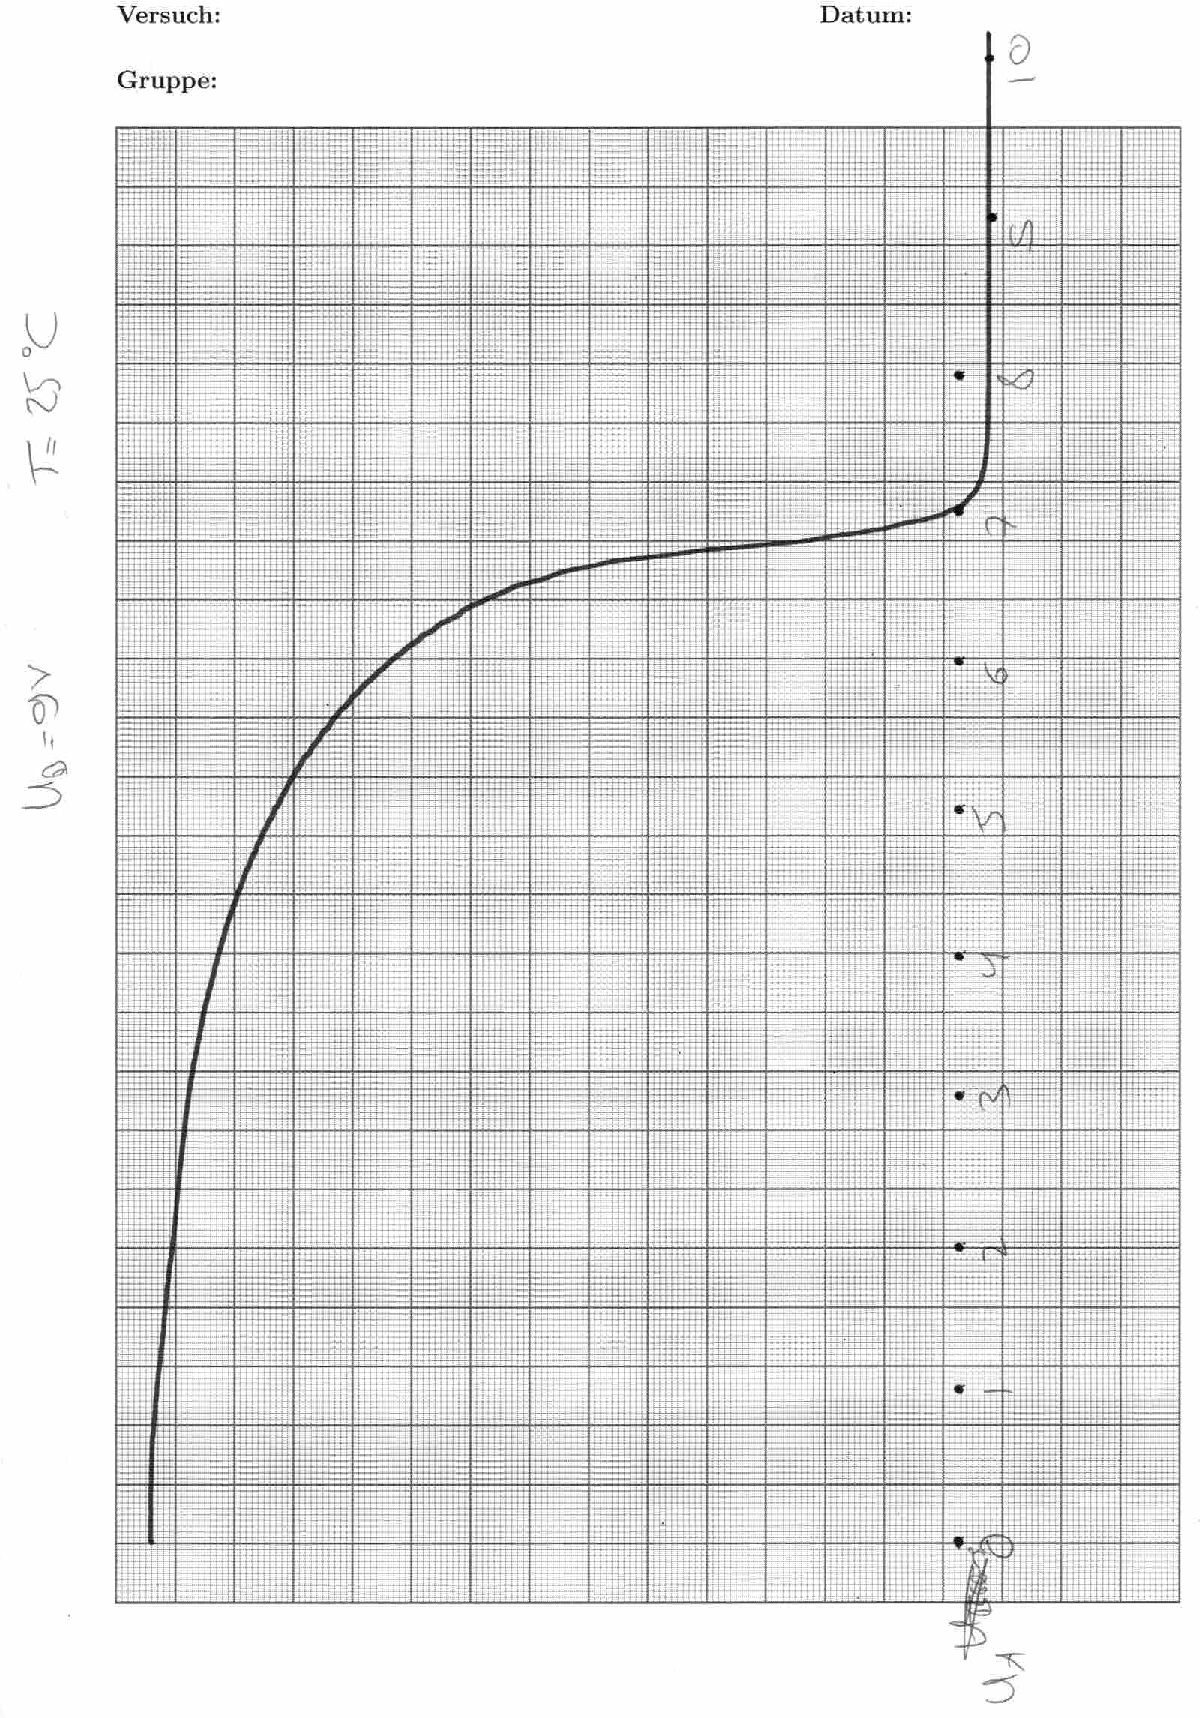
\includegraphics[width=0.8\textwidth]{Daten/0025.jpg}
	\caption{Original Messdaten zu $\SI{25}{\celsius}$.}
\end{figure}
\begin{figure}
	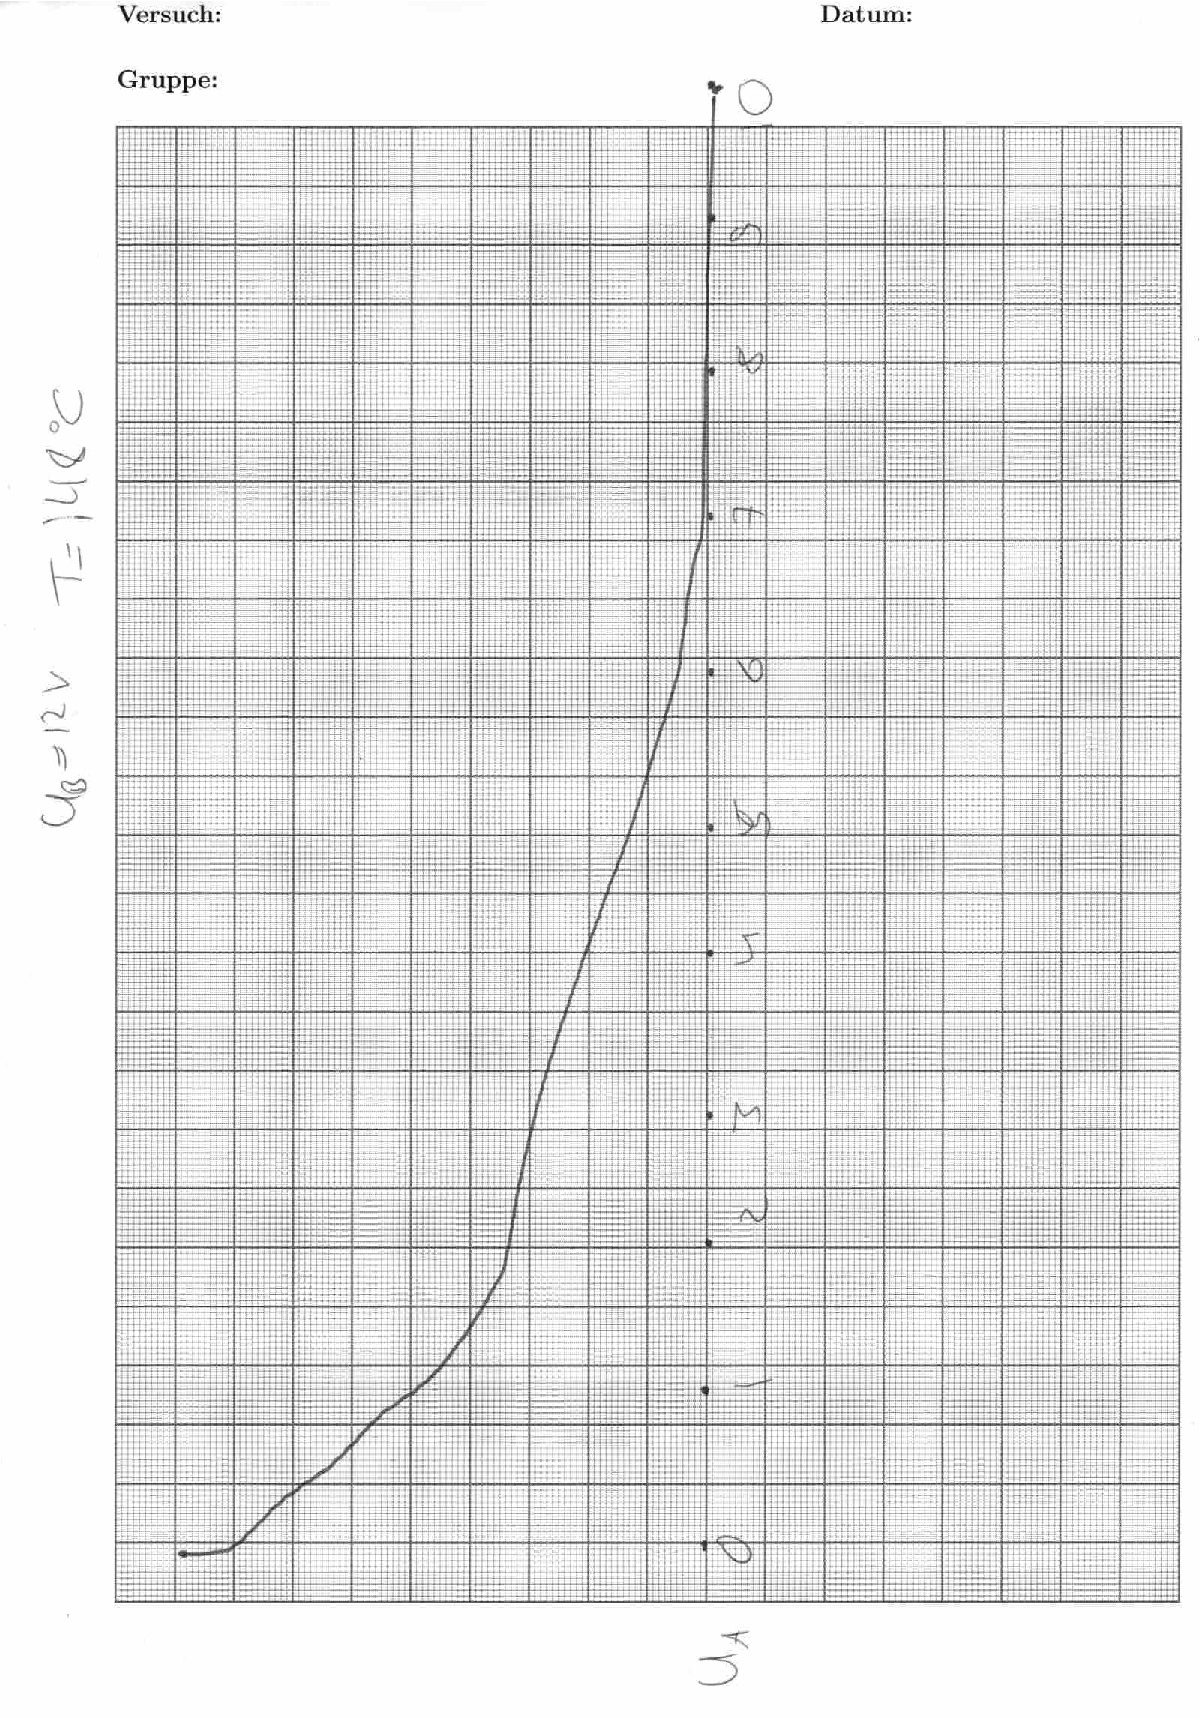
\includegraphics[width=0.8\textwidth]{Daten/1480.jpg}
	\caption{Original Messdaten zu $\SI{148}{\celsius}$.}
\end{figure}
\begin{figure}
	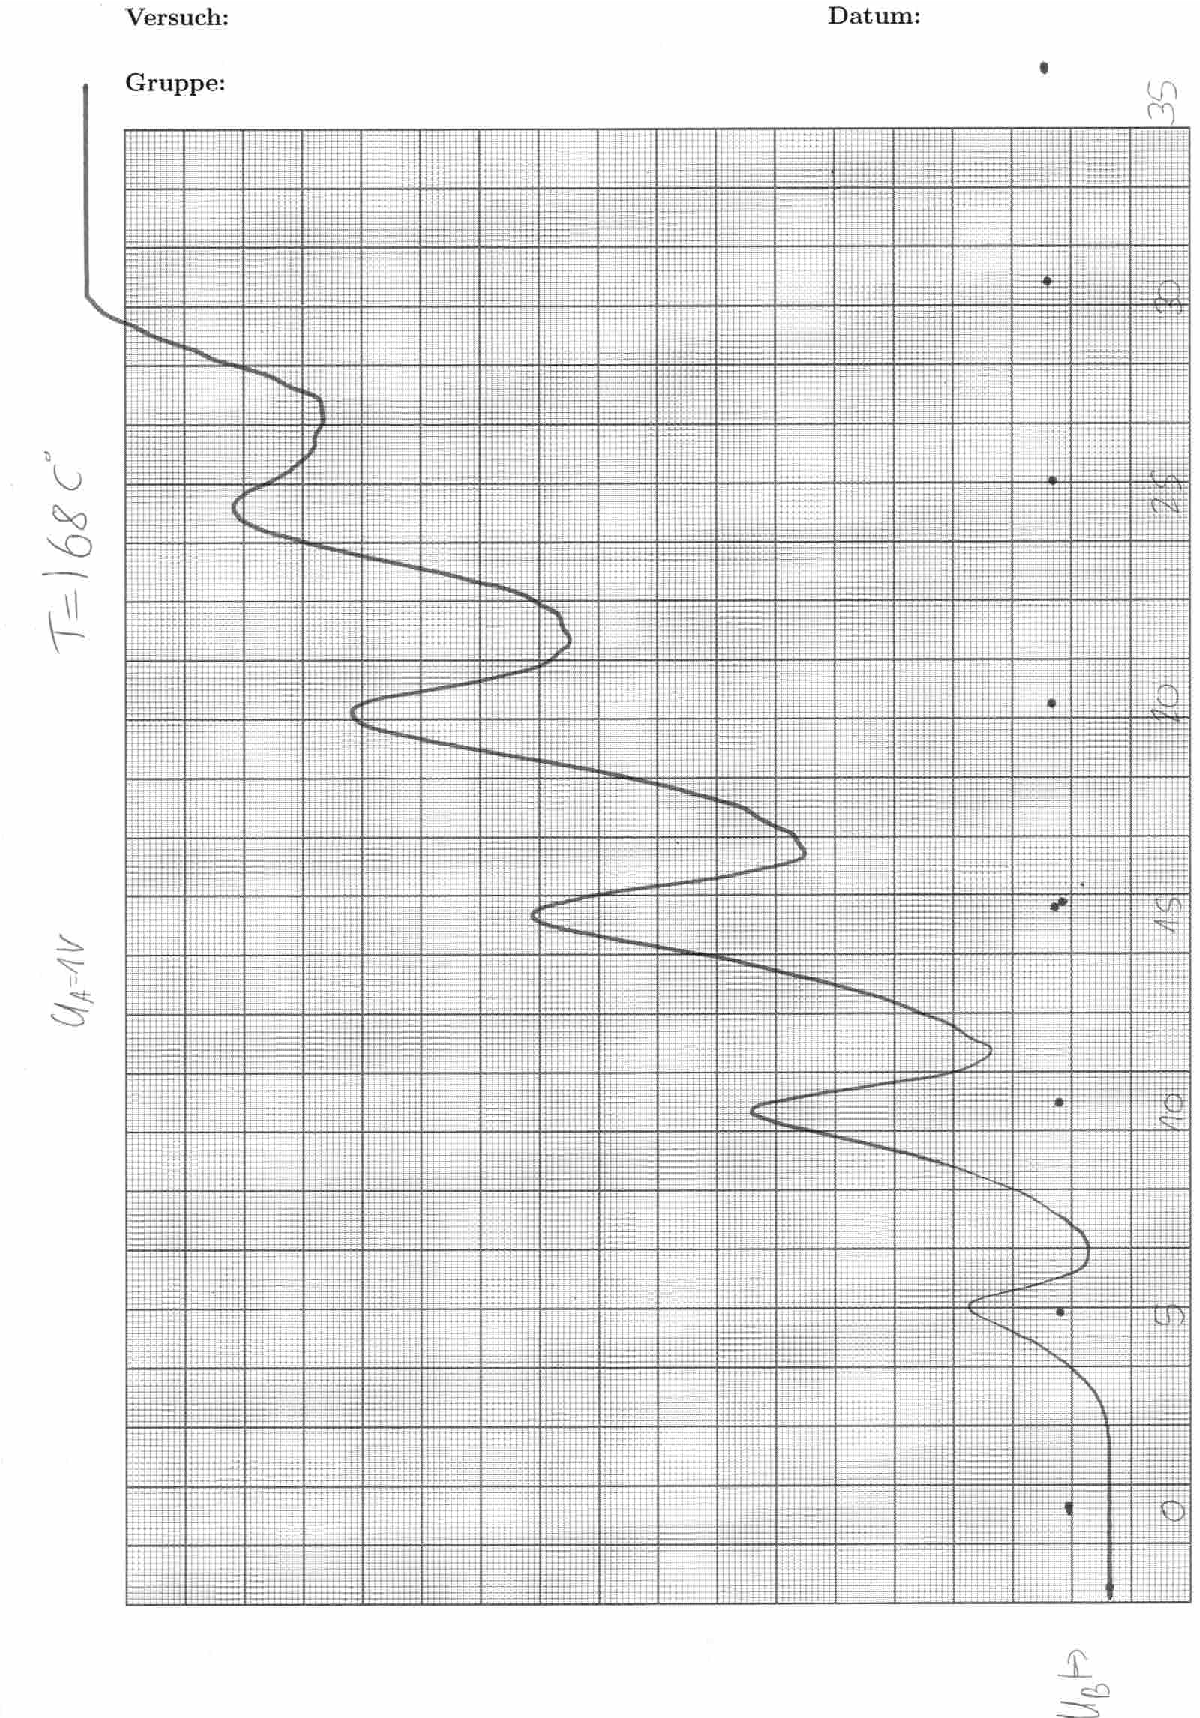
\includegraphics[width=0.8\textwidth]{Daten/1680.jpg}
	\caption{Original Messdaten zu $\SI{168}{\celsius}$.}
\end{figure}
\begin{figure}
	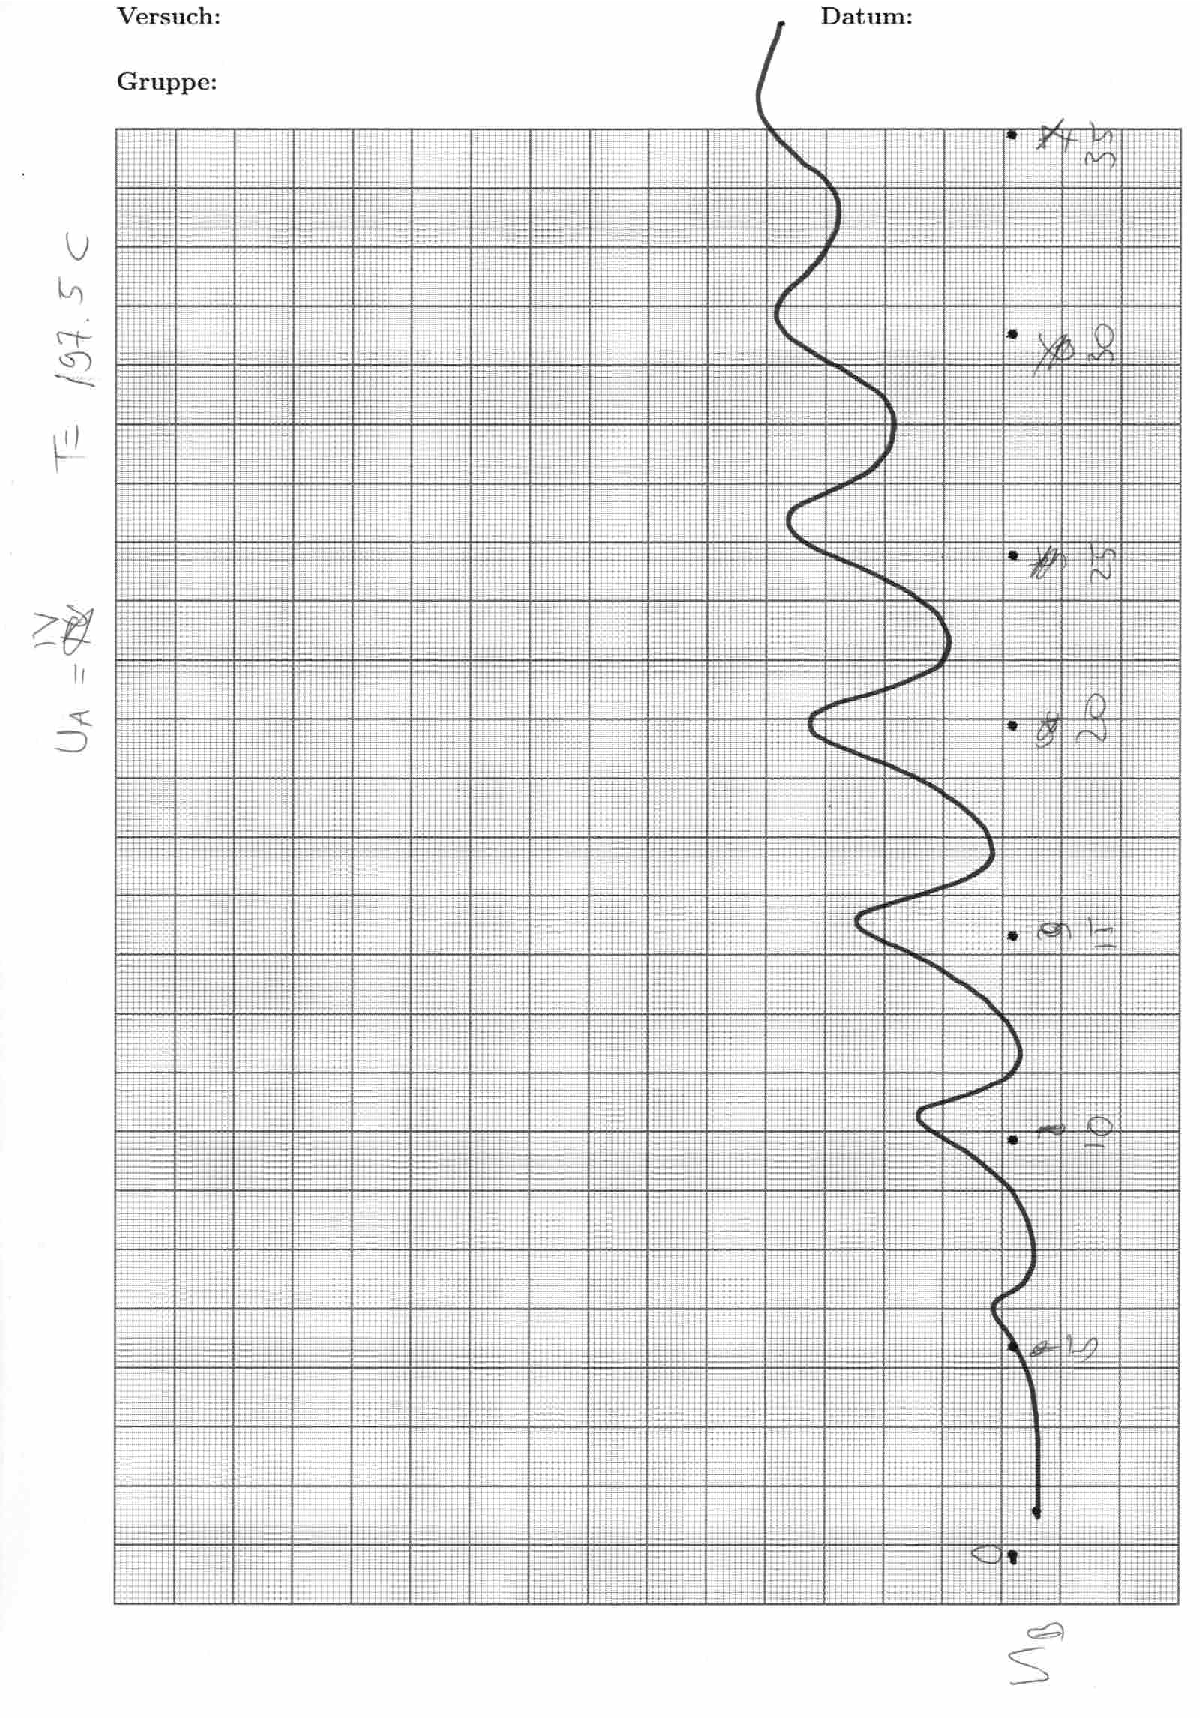
\includegraphics[width=0.8\textwidth]{Daten/1975.jpg}
	\caption{Original Messdaten zu $\SI{197.5}{\celsius}$.}
\end{figure}

\end{document}
